\subsection*{Problema 03}

\textbf{Enunciado:} Probar que si $0 < x < y$, 
entonces se cumple la desigualdad:
\begin{equation*}
\dfrac{1}{y} < \dfrac{\ln y - \ln x}{y - x} < \dfrac{1}{x}
\end{equation*}

\textbf{Solución:} 
Para demostrar la desigualdad propuesta, 
utilizamos el Teorema del Valor Medio 
de Lagrange. 

Consideremos la función real 
$f(t) = \ln(t)$. 
Esta función es continua en el intervalo 
cerrado $[x, y]$ y derivable en el 
intervalo abierto $(x, y)$, 
dado que $0 < x < y$.

Por el Teorema del Valor Medio, 
existe al menos un número $c$ en el 
intervalo $(x, y)$ tal que:
\begin{align*}
f'(c) &= \dfrac{f(y) - f(x)}{y - x}
\end{align*}

Calculamos la derivada de la función 
$f(t)$:
\begin{align*}
f'(t) &= \dfrac{1}{t}
\end{align*}

Evaluando la derivada en el punto $c$, 
obtenemos $f'(c) = \dfrac{1}{c}$. 
Sustituyendo esto en la expresión del 
teorema, junto con $f(y) = \ln(y)$ y 
$f(x) = \ln(x)$, resulta:
\begin{align*}
\dfrac{1}{c} &= \dfrac{\ln y - \ln x}{y - x}
\end{align*}

Como se sabe que el valor $c$ pertenece 
al intervalo abierto $(x, y)$, 
se cumple la siguiente desigualdad 
estricta para sus inversos:
\begin{align*}
x < c < y \implies \dfrac{1}{y} < \dfrac{1}{c} < \dfrac{1}{x}
\end{align*}

Finalmente, sustituyendo la expresión 
de la derivada evaluada en $c$ dentro 
de esta cadena de desigualdades, 
obtenemos el resultado deseado:
\begin{align*}
\dfrac{1}{y} < \dfrac{\ln y - \ln x}{y - x} < \dfrac{1}{x}
\end{align*}
Esto completa la demostración.

\begin{figure}[H]
	\centering
	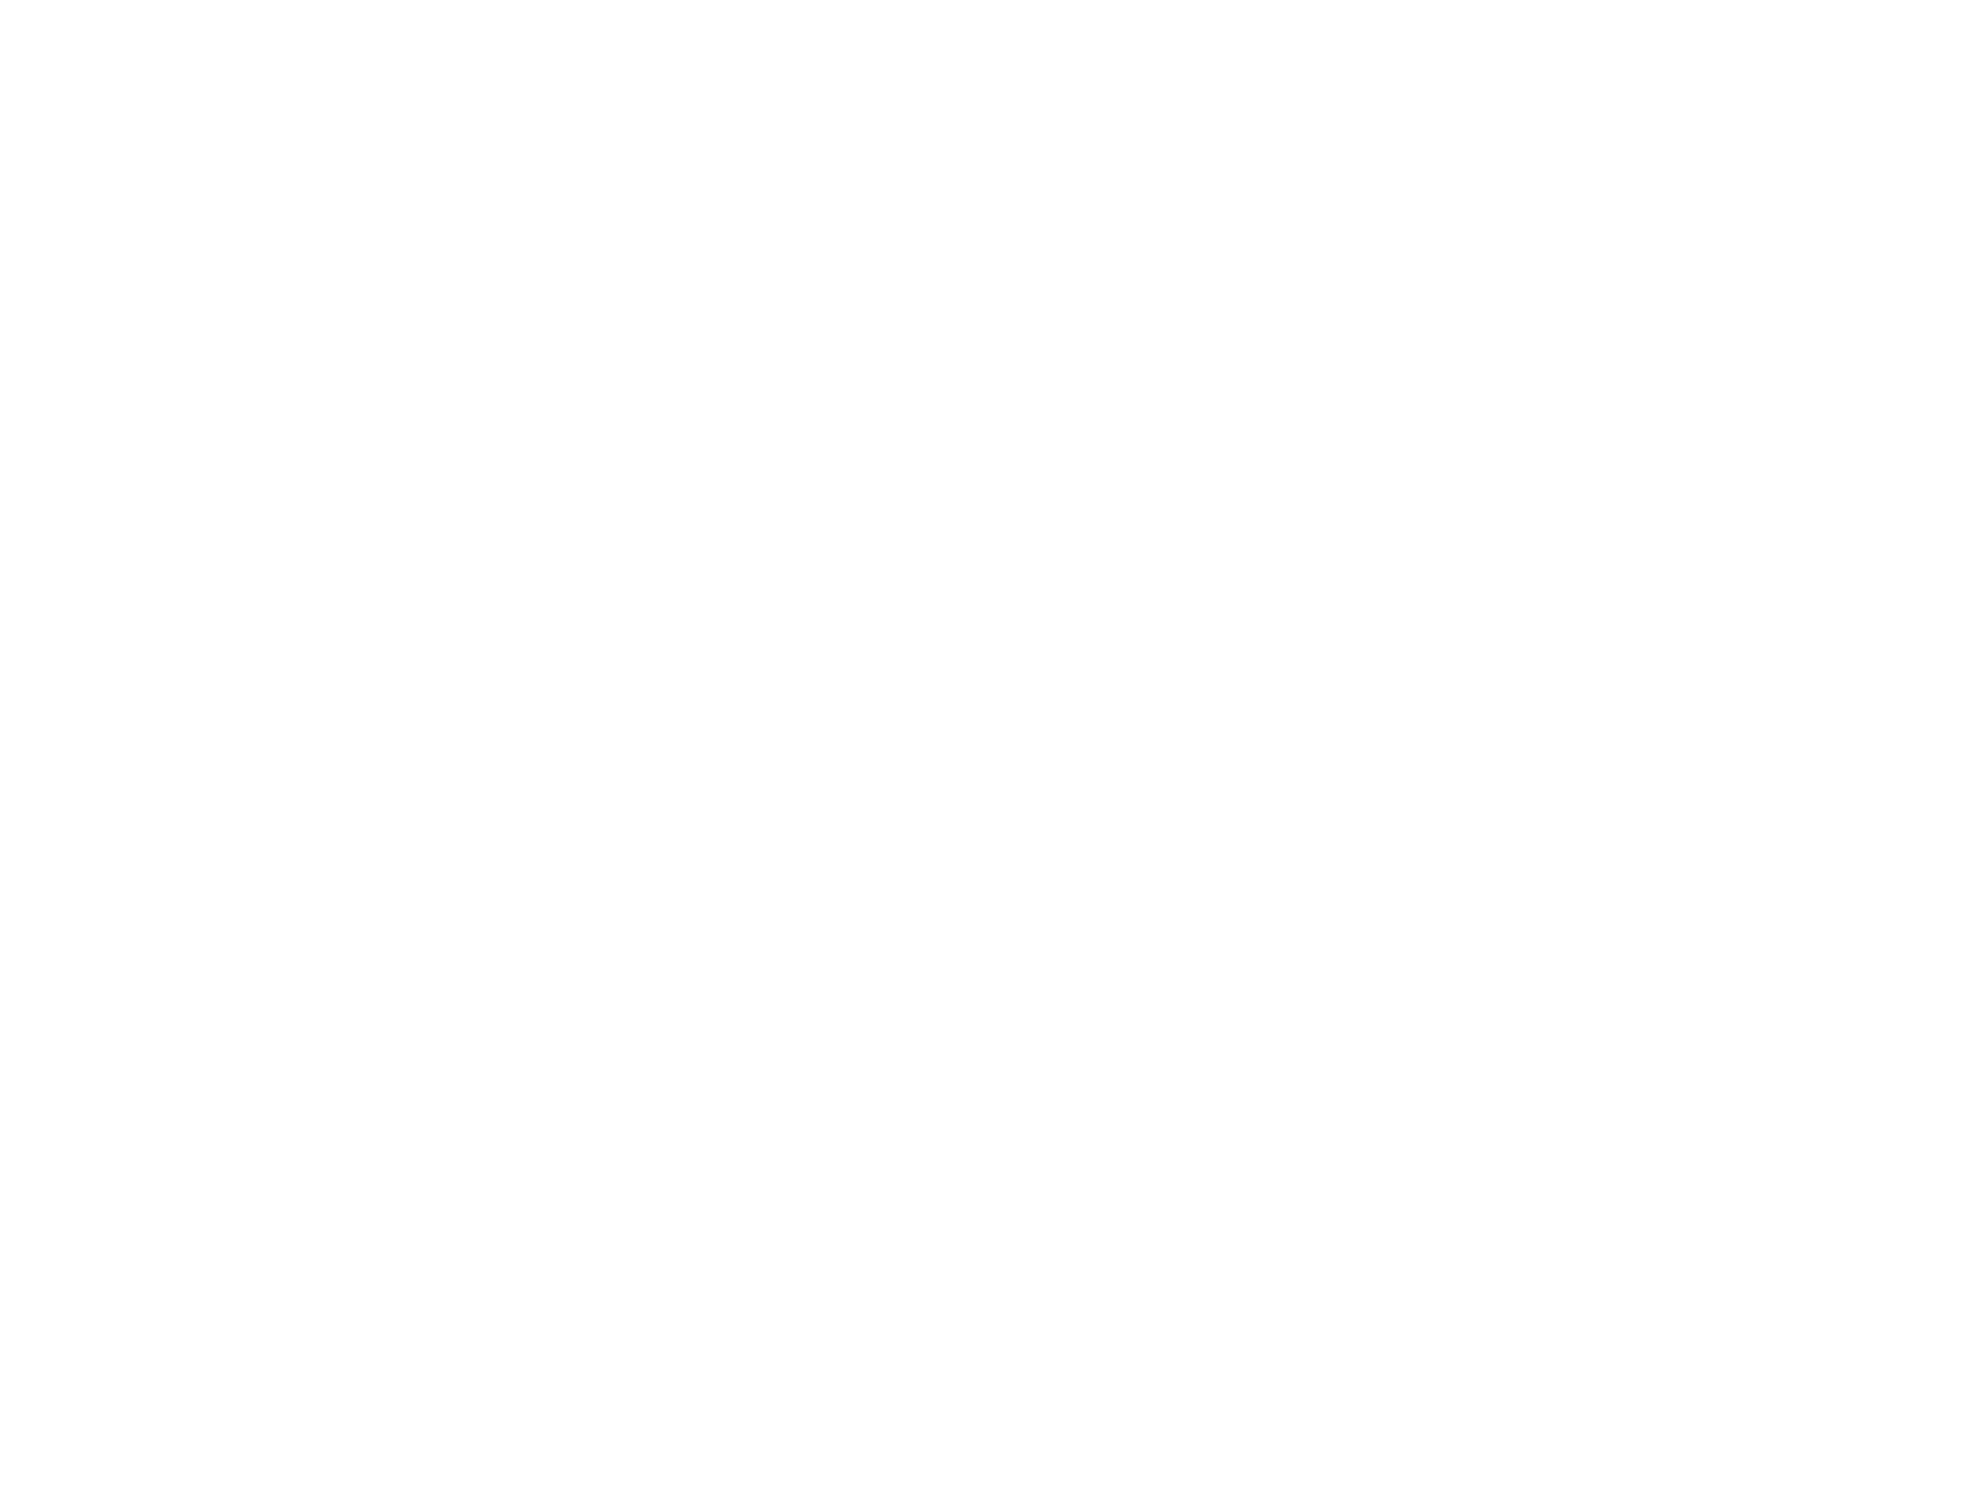
\includegraphics[width=\columnwidth]{semana_08/graficas/SEM08_P03_grafica.png}
	\caption{Representación gráfica de $f(x)$ y su antiderivada $F(x)$ evaluada para la constante de integración $C = 0$ (Problema 03).}
	\label{fig:problema03}
\end{figure}
